\documentclass[10pt,letterpaper,extrafontsizes]{memoir}
\listfiles
\usepackage{comment}

\usepackage{memsty}
%%%%%%%%%%%%%%%%%%%%%%%%%%%%
\usepackage{titlepages}  % code of the example titlepages
\usepackage{memlays}     % extra layout diagrams
\usepackage{dpfloat}     % floats on facing pages
\usepackage{fonttable}[2009/04/01]   % font tables
\usepackage{longtable}
\setlength{\doublerulesep}{0pt}
\newcommand{\myhline}{\hline\hline\hline}

%%%%%%%%%%%%%%%%%%%%%%%%%%%%

%%%% Use the built-in division styling
\headstyles{memman}

%%% ToC down to subsections
\settocdepth{subsection}
%%% Numbering down to subsections as well
\setsecnumdepth{subsection}

%%%% extra index for first lines
\makeindex[lines]

% this 'if' is used to determine whether we are compiling the memoir
% master in the subversion repository, or the public memman.tex
\newif\ifMASTER
\MASTERfalse
%\MASTERtrue

\ifMASTER

% we add this to the first page of each chapter

\makepagestyle{chapter}
\makeoddfoot{chapter}{\addRevisionData}{\thepage}{}
\makeevenfoot{chapter}{\addRevisionData}{\thepage}{}

\else
% disable svn info collecting
\newcommand\svnidlong[4]{}
\fi

\setsecheadstyle{\Large\normalfont}
\setbeforesecskip{-1\onelineskip plus -1ex minus -.2ex}
\setaftersecskip{1\onelineskip plus .2ex}
\setsubsecheadstyle{\centering\normalfont}
\setbeforesubsecskip{-1\onelineskip plus -1ex minus -.2ex}
\setaftersubsecskip{1\onelineskip plus .2ex}

\OnehalfSpacing \OnehalfSpacing*

\setsubsecheadstyle{\normalfont}


%% end preamble
%%%%%%%%%%%%%%%%%%%%%%%%%%%%%%%%%%%%%%%%%%%%%%%%%%%%%%%
%#% extend

\usepackage[draft]{fixme}
\fxsetup{
  layout=marginnote
} 

\chapterstyle{ger}

\title{ \textsc{\huge MU User Manual} \\ \textsc{A guide to using MU middleware} \\ \textsc{\small v 1.0}}
\author{UNIZG}

\begin{document}

\maketitle
\thispagestyle{empty}
%%%%%%%%%%%%%%%%%%%%%%%%%%%%%%%%%%%%%%%%%%%%%%%%%%%%%%%

\chapter{Connecting to aMussel over Bluetooth}
\label{ch:connecting_to_ble}

\begin{figure}[htb]
    \centering
	  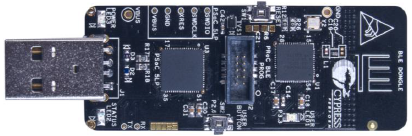
\includegraphics[width=0.5\linewidth]{figures/USB_Dongle.png}
	\caption{BLE USB dongle (CY5670)}
	\label{fig:ble_hardware}
\end{figure}

Necessary hardware components:
\begin{itemize}
	\item Bluetooth (BLE) module on MainBoard (MB) -- each aMussel comes with an embedded BLE module
	\item BLE dongle that needs to be connected to user's PC USB port -- \href{http://www.cypress.com/documentation/development-kitsboards/cy5670-cysmart-usb-dongle}{dongle used for subCULTron} \\
	The purpose of BLE dongle is to provide UART bridge between MB and PC. It's main purpose is to establish basic serial communication between MB on aMussel and PC.
\end{itemize}

In order to connect to aMussel over Bluetooth, the following prerequisites have to be met:
\begin{enumerate}
	\item BLE dongle has to be programmed.
	\item BLE module on MB has to be programmed with a certain aMussel ID.
\end{enumerate}

\section{Programming BLE dongle}

The code for BLE dongle is provided in subCULTron's GitHub page (\href{https://github.com/subCULTron-project}{link}), \texttt{BLE-Dongle} repository. To program BLE dongle you need to install PSoC Creator 4.0 IDE (\href{http://www.cypress.com/documentation/software-and-drivers/psoc-creator-software-archive}{here}) and checkout the needed git repository.

Then:
\begin{enumerate}
	\item Open the \texttt{BLE-Dongle} project in PSoC Creator. Build the project (right click on project name > Build \texttt{BLE\_DONGLE}).
	\item Set \texttt{BLE\_DONGLE} project to active (right click on project name > Set As Active Project).
	\item Connect BLE dongle to the PC's USB port 
	\item Program the dongle (\textit{program} button in PSoC creator or Ctrl+F5).
	\item If prompted, select a device to program.
\end{enumerate}

\section{Programming BLE module}

BLE module can be programmed using MiniProg programmer. The code is provided in \texttt{BLE\_UART\_BRIDGE} project of PSoC creator \texttt{MU31S-000} workspace, which can be found on project's GitHub page, \texttt{MainBoard-middleware} repository.

\begin{figure}[htb]
    \centering
	  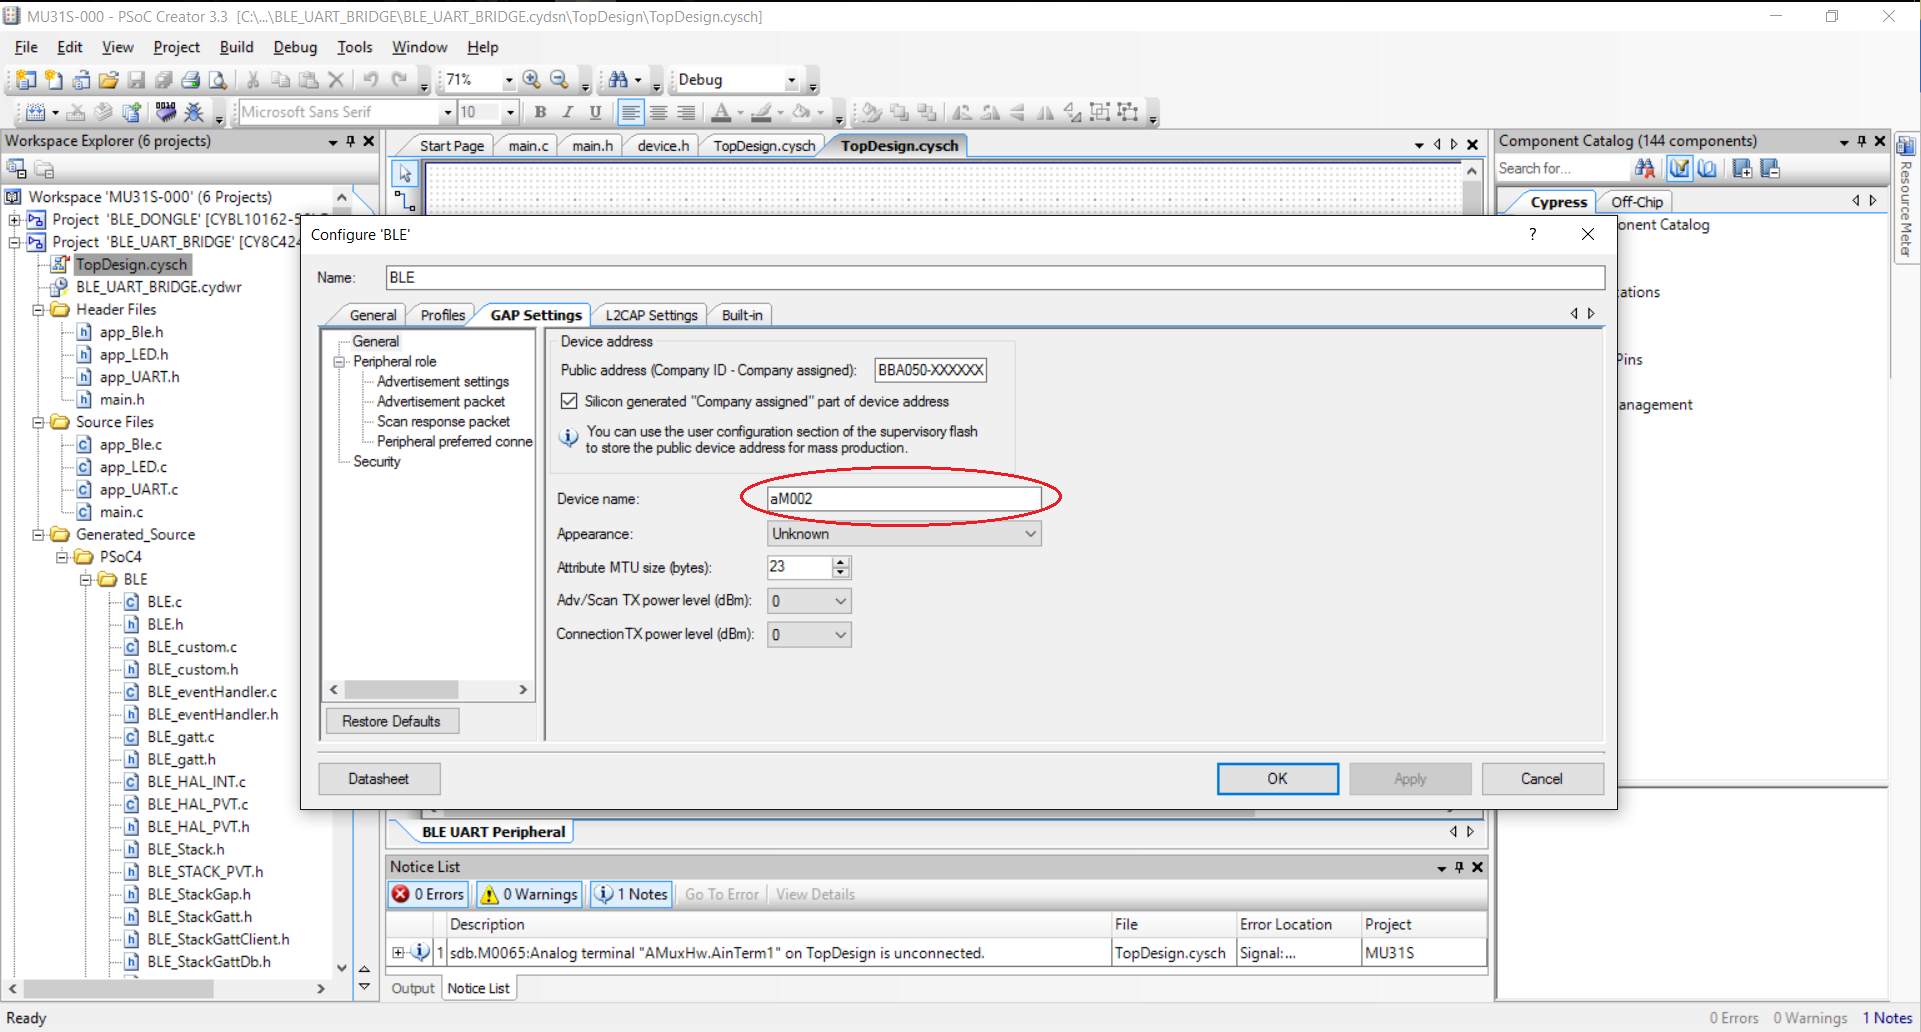
\includegraphics[width=\linewidth]{figures/BLE_device_name.PNG}
	\caption{Setting the BLE device name}
	\label{fig:ble_device_name}
\end{figure}

Steps:
\begin{enumerate}
	\item Modify the project to define aMussel ID. To do so, open TopDesign.cysch and double click on BLE module. Go to GAP Settings > General and enter aMussel ID in Device Name field (see Figure \ref{fig:ble_device_name}). Naming convention is as follows: \texttt{'aMXXX'}, where \texttt{'XXX'} represents aMussel ID in range $[000-999]$, e.g. \texttt{'aM001', 'aM023'} \ldots
	\item Build the project (right click on project name > Build \texttt{BLE\_UART\_BRIDGE}).
	\item Set \texttt{BLE\_UART\_BRIDGE} project to active (right click on project name > Set As Active Project).
	\item Connect MiniProg to BLE module and the PC.
	\item Program the device (\textit{program} button in PSoC creator or Ctrl+F5).
	\item If prompted, select a device to program.
\end{enumerate}

\section{Communicating with MU using BLE}

\begin{figure}[htb]
    \centering
	  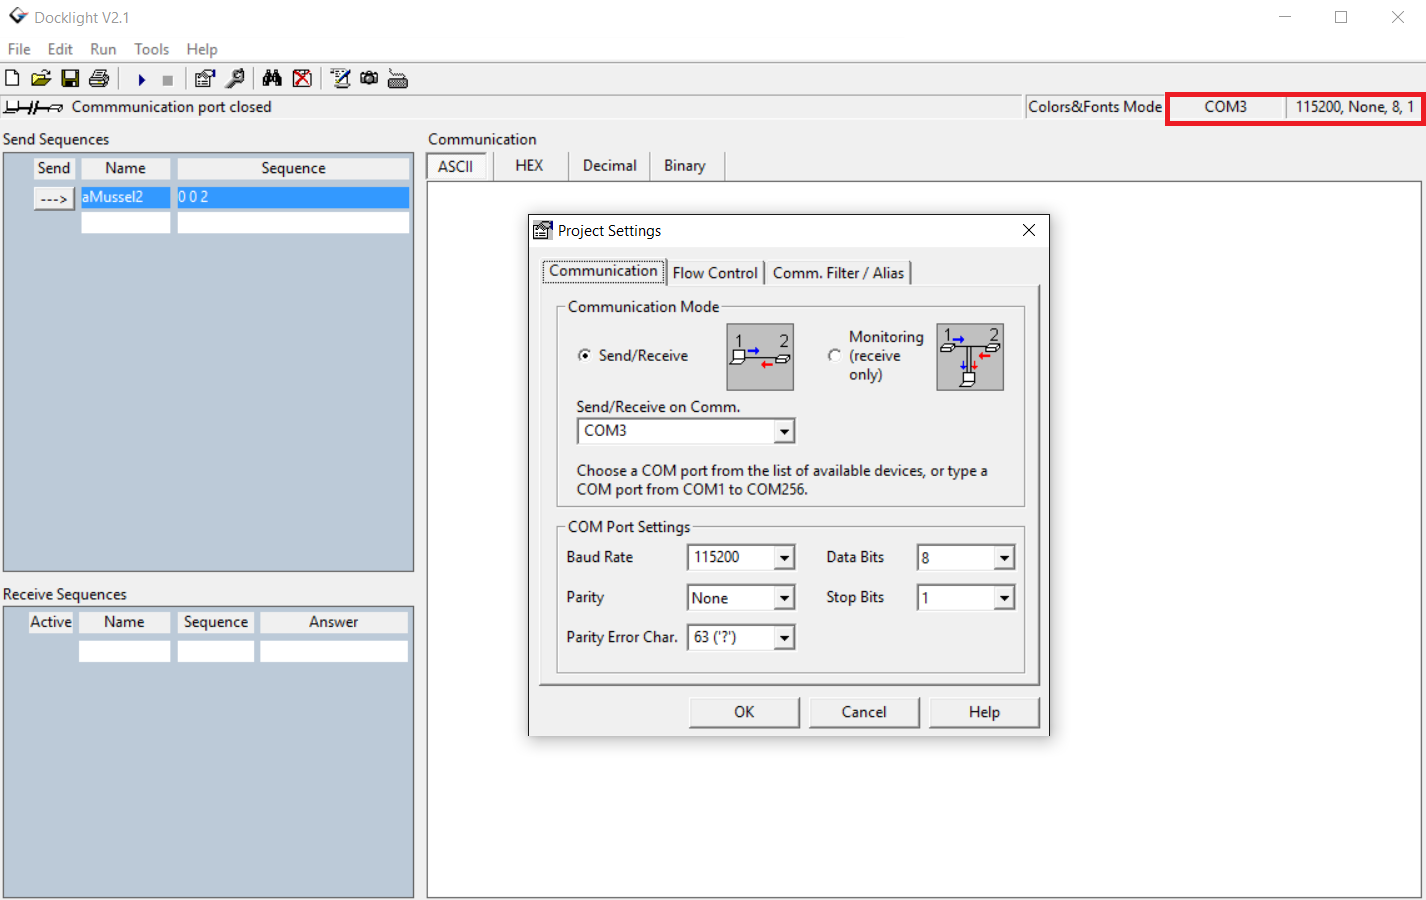
\includegraphics[width=\linewidth]{figures/Docklight_COM.PNG}
	\caption{Selecting the COM port}
	\label{fig:docklight_com}
\end{figure}

\begin{figure}[htb]
    \centering
	  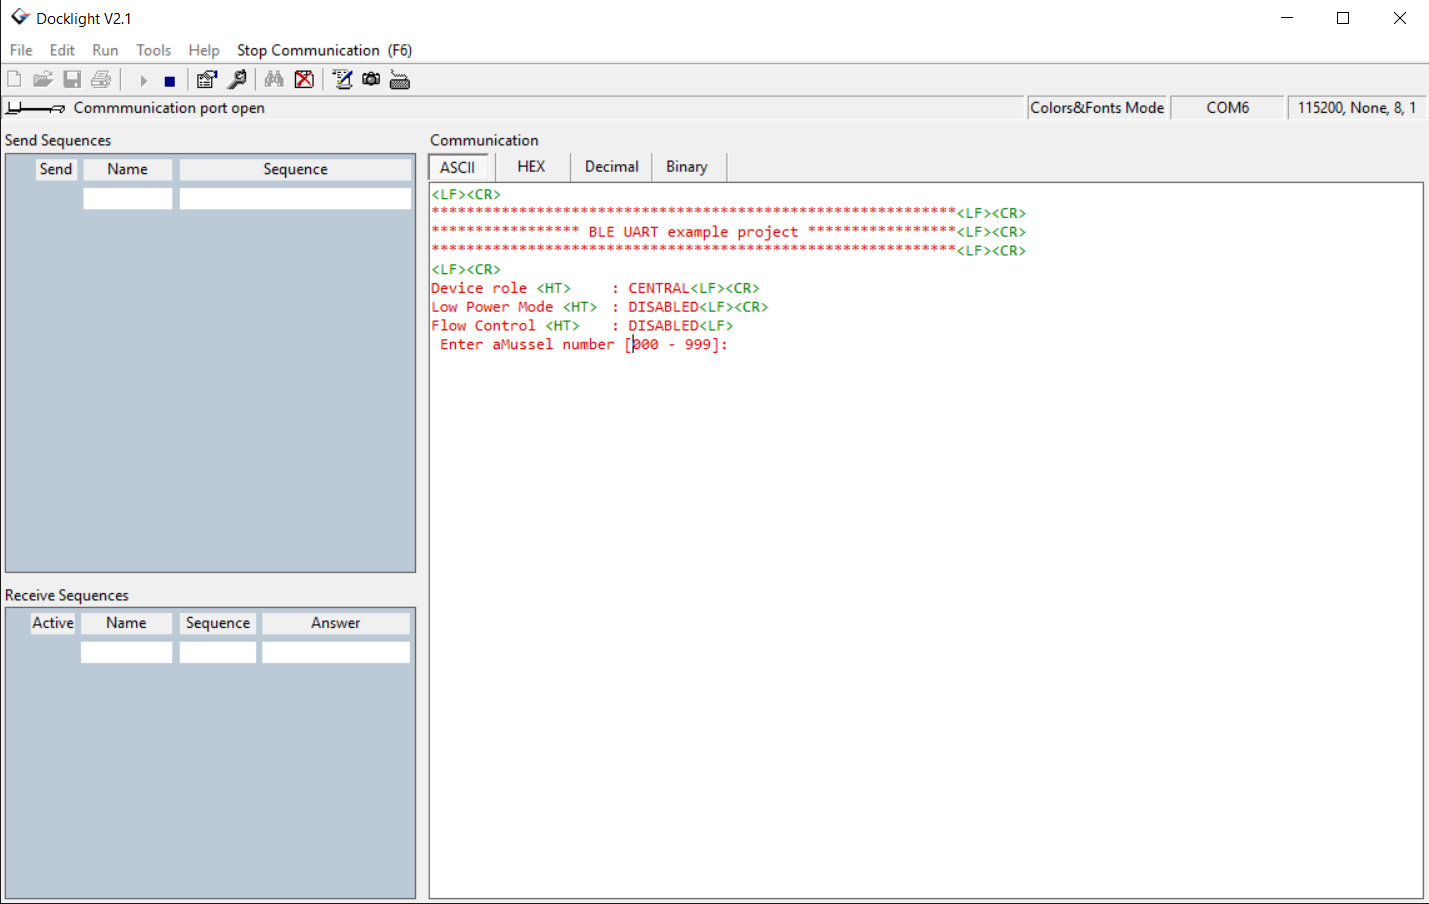
\includegraphics[width=\linewidth]{figures/Docklight_BLE_dongle.PNG}
	\caption{BLE bridge status}
	\label{fig:docklight_ble_bridge_status}
\end{figure}

\begin{figure}[htb]
    \centering
	  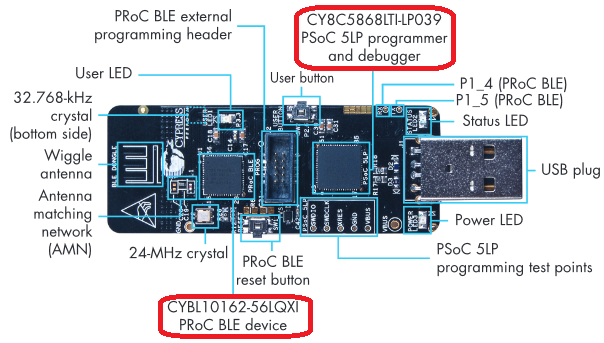
\includegraphics[width=0.6\linewidth]{figures/USB_dongle_parts.png}
	\caption{CY5670 USB Dongle}
	\label{fig:usb_dongle_parts}
\end{figure}

\begin{figure}[htb]
    \centering
	  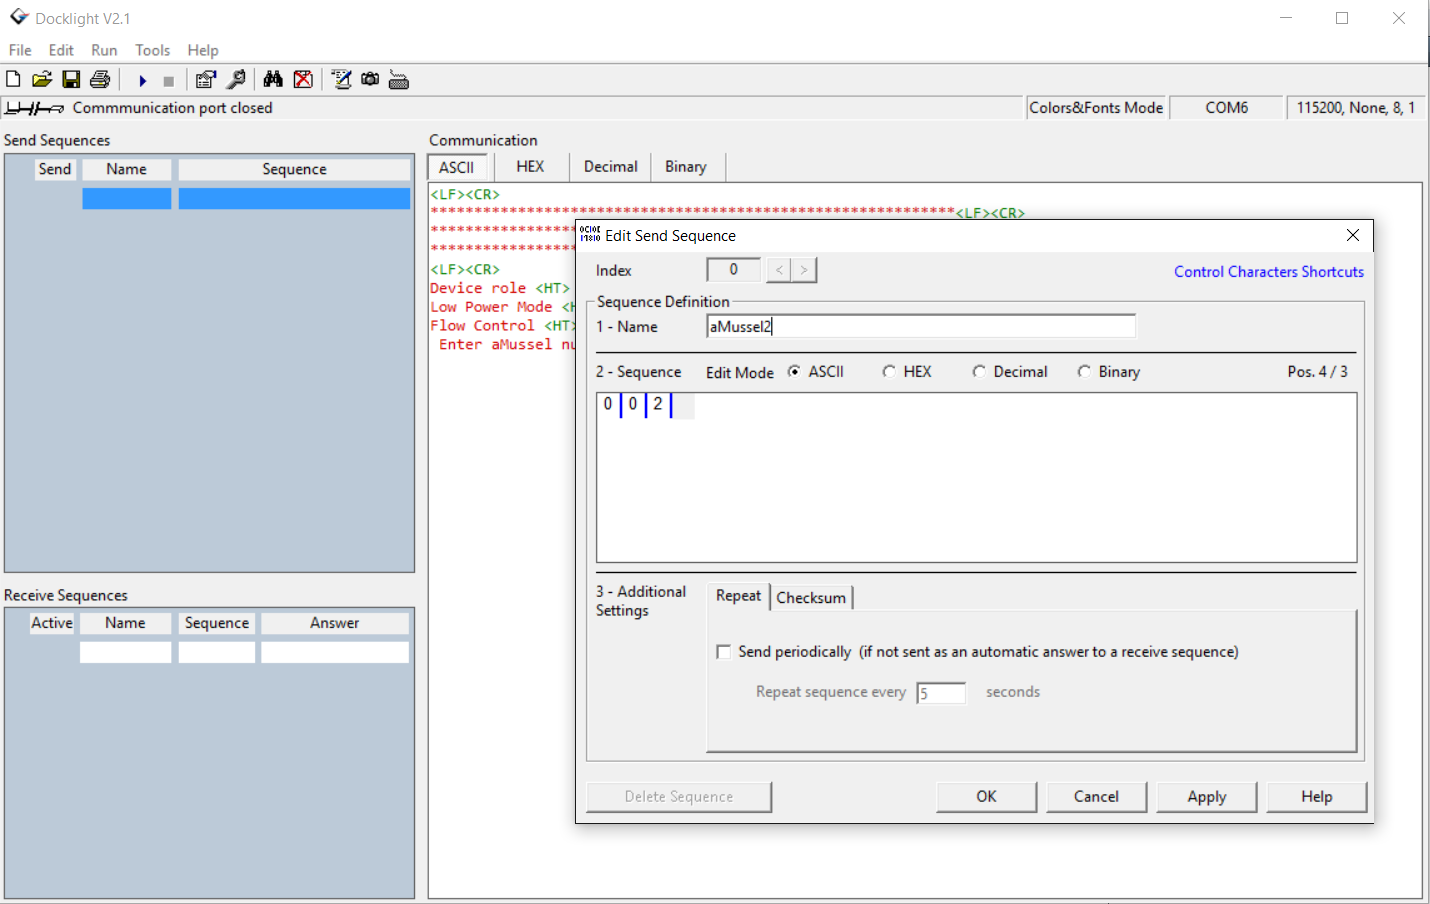
\includegraphics[width=\linewidth]{figures/Docklight_aMussel_selection.PNG}
	\caption{Selecting a device to connect to}
	\label{fig:docklight_aMussel_selection}
\end{figure}

To successfully send and receive data between aMussel and PC, we recommend the following setup:
\begin{enumerate}
	\item Connect the programmed BLE dongle to your PC.
	\item Open Docklight \footnote{\url{docklight.de/}} (or any other tool for serial communication).
	\item Connect to the correct COM port. Port can be selected by double clicking on top right sections of status bar (indicated with red rectangle in Figure \ref{fig:docklight_com}). After selecting the port, make sure the settings are matching the ones in the figure. Now you can simply press the play button to establish connection.
	\item When connected to BLE dongle, you should see the output in your serial communication program as presented in Figure \ref{fig:docklight_ble_bridge_status}. If the output is not there or the program is stuck for any reason, you can always reset it by pressing the user button on dongle (see Figure \ref{fig:usb_dongle_parts}).
	\item The next step is to select device ID you wish to connect to. You do so by sending a sequence representing device's unique identifier. For example, if BLE board on aMussel is programmed to have ID \texttt{001}, the sequence needs to match it. For reference, look at Figure \ref{fig:docklight_aMussel_selection}.
	\item Upon connection establishment the program prints out: \\
	\hspace{10pt}\parbox[t]{\linewidth}{\texttt{Server with matching custom service discovered... \\
		Connection established \\
		Notifications enabled \\
		Start entering data:
	}}
	\item Now the connection is established and you can start sending and receiving data.
\end{enumerate}

\chapter{Programming using Bootloader}

\emph{Bootloader} is a short program used to burn the firmware to the microcontroller without any programmer device. It is the first thing to run on device power on and is accessible through the serial interface.

\section{USB connection (obsolete)}

Setup described in this section enables you to program Main Boards using wired connection (i.e. mini USB cable) Bootloader.

\subsection{Programming the Bootloader on Main Board}
\label{subsec:programming_the_bootloader}

A prerequisite to using Bootloader to program the Main Board is having the Bootloader itself configured and programmed onto the board. USB (wired) Bootloader is provided in \texttt{UART\_BOOTLOADER} project of PSoC creator \texttt{MU31S-000} workspace.

Steps:
\begin{enumerate}
	\item Build the project (right click on project name > Build \texttt{UART\_BOOTLOADER}).
	\item Set \texttt{UART\_BOOTLOADER} project to active (right click on project name > Set As Active Project).
	\item Connect MiniProg to MB and the PC.
	\item Program the MB (\textit{program} button in PSoC creator or Ctrl+F5).
	\item If asked, select a device to program. Sometimes the connection between MB and MiniProg is bad so make sure you adjust the cable until the device \texttt{PSoC 5LP CY8C5888LTI*-LP097} is detected. %TODO version??
	\item Once the device is detected, select \texttt{Port Acquire} > \texttt{Connect} > \texttt{OK} and wait for the completion of programming process.
\end{enumerate}

\subsection{Programming MB using Bootloader}
\label{subsec:programming_with_bootloader}

In order to program Main Board using Bootloader, \texttt{Bootloadable} component on MB has to be running and awaiting for programming request. It can be achieved by setting a waiting time after each system power on during which MB enters this mode. It is, however, not efficient because we sometimes need to program MB without power cycling it. Therefore, programs devised for Main Board always need to have one \textit{interpreter} task running which activates Bootloadable on request. This mode is entered by sending \texttt{'b'} character to MB's general purpose (debugging) UART.

\begin{figure}[htb]
    \centering
	  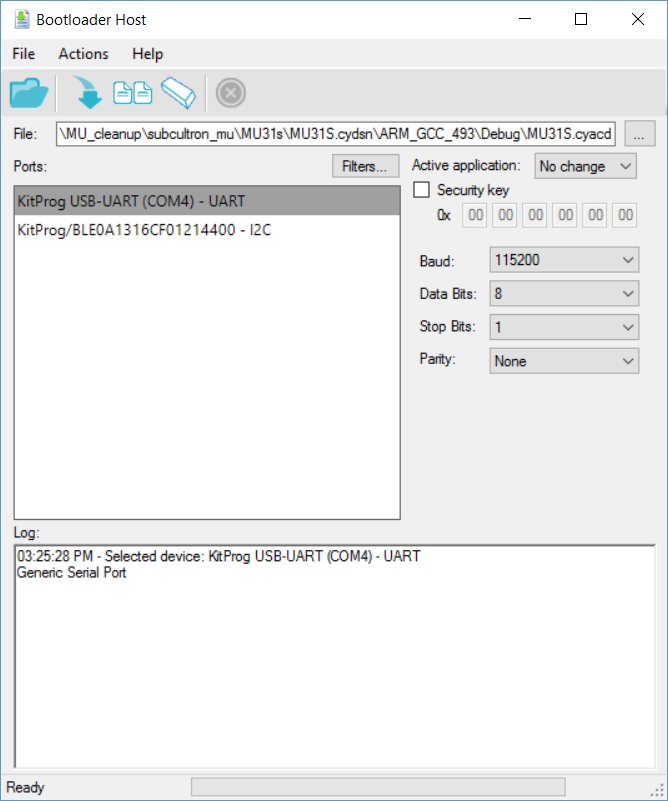
\includegraphics[width=0.6\linewidth]{figures/Bootloader_BLE.png}
	\caption{Setting up Bootloader Host}
	\label{fig:bootloader_host}
\end{figure}

The next step is to connect to the Main Board and start the programming process.\\
Steps:
\begin{enumerate}
	\item Connect the MB to your PC via mini USB cable. Make sure all connections to this COM port are closed (stop connections in Docklight).
	\item Open the project you wish to program in PSoC Creator.
	\item Go to \texttt{Tools} > \texttt{Bootloader Host}.
	\item Select the correct COM port and adjust settings to match the ones in Figure \ref{fig:bootloader_host}.
	\item Click on \texttt{Program} button and wait for the process to execute.
\end{enumerate}

\section{BLE Bootloader}

The process of programming MB using BLE Bootloader is the same as the one using wired connection Bootloader. The only difference is in the way the connection to the device is established (step 1 in the previous section). For guide on setting up BLE bridge between MB and PC, refer to Chapter \ref{ch:connecting_to_ble}. Bootloader project that needs to be programmed onto the Main Board is \texttt{UART\_Bootloader\_BLE}.

\section{I2C Bootloader}

...
%\chapter{Setting up environment}
\label{ch:env_setup}

To set up testing/scenario environment, a special header file \texttt{device.h}, has to be modified. As we can see in Figure \ref{fig:device_h}, all of devices used in program are specified using binary flags which denote their presence/absence in scenario in question.

\begin{figure}[htb]
    \centering
	  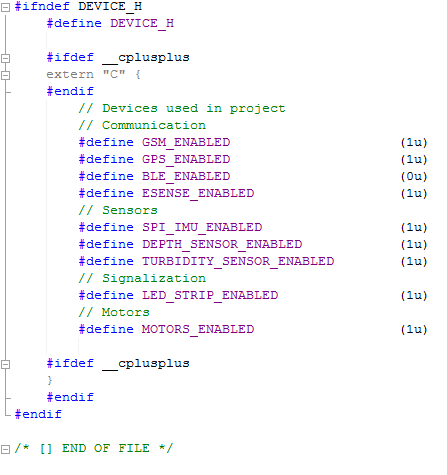
\includegraphics[width=0.7\linewidth]{figures/Environment_setup.png}
	\caption{Example setup of device.h}
	\label{fig:device_h}
\end{figure}

In testing scenarios, the most important parameter is \texttt{BLE\_ENABLED} which also specifies the output of debugging messages as well as the expected source of commands. Therefore, if \texttt{BLE\_ENABLED} is set to \texttt{0}, all of the testing is done through wired UART (i.e. USB cable), otherwise the input is expected to come from BLE device.
\chapter{Testing device functionality}
\label{ch:testing_device_fun}

For individual device functionality test a special task which interprets commands sent through serial port and calls corresponding API functions has been devised. It is called \texttt{test\_function} and is located in \texttt{main.c} of \texttt{MU31S} project.

To send commands, a serial connection to MB's general purpose UART needs to be established. All of the commands and debugging messages are then sent through that link.

To test the functionality, a special sequence of messages has been defined. The controls are found in the table \ref{tbl:mu_comms}.

\begin{longtable}[c]{llll}
	\caption{MB testing commands} \label{tbl:mu_comms} \\
	    \myhline
    	\multicolumn{4}{l}{Bootloader} \\ \hline
	    b & ~ & ~ & enter Bootloader \\
	    \myhline
	    \multicolumn{4}{l}{Power board} \\ \hline
	    P & 1 & ~ & switch to main battery \\
   	    P & 2 & ~ & switch to backup battery \\
   	    P & 3 & ~ & disable charging \\
   	    P & 4 & ~ & get main battery voltage \\
   	    P & 5 & ~ & get backup battery voltage \\
   	    P & 6 & ~ & get main battery current \\
   	    P & 7 & ~ & get backup battery current \\
   	    P & 8 & ~ & get supply current \\
   	    P & 9 & ~ & get main battery's charging status \\
   	    P & A & ~ & get backup battery's charging status \\
   	    P & B & ~ & enable charging \\
		\myhline
        \multicolumn{4}{l}{Electric sense} \\ \hline
	    e & b & ~ & esense board program \\
	    e & 0 & ~ & esense board init \\
	    e & s & ~ & esense board 's' command \\
	    e & m & ~ & esense board 'm' command \\
	    e & + & ~ & esense board '+' command \\
	    e & - & ~ & esense board '-' command \\
	    e & a & ~ & esense board get angle \\
	    e & d & ~ & esense board get distance \\
	    \myhline
        \multicolumn{4}{l}{Turbidity sensor} \\ \hline
	    t & ~ & ~ & Get turbidity sensor reading. \\
	    \myhline
        \multicolumn{4}{l}{GSM/GPS module} \\ \hline
	    g & c & ~ & call a number defined in test function \\
   	    g & h & ~ & hang up \\
   	    g & s & ~ & send SMS to a number defined in test function \\
   	    g & m & ~ & receive SMS \\
   	    g & u & ~ & list all unread SMS \\
   	    g & a & ~ & list all SMS \\
   	    g & l & ~ & clean read SMS \\
   	    g & N & ~ & power on GPS module \\
   	    g & F & ~ & power off GPS module \\
   	    g & f & ~ & get GPS fix status \\
   	    g & k & ~ & get GPS data \\
   	    \myhline
        \multicolumn{4}{l}{SPI IMU} \\ \hline
	    p & a & ~ & get accelerometer data \\
   	    p & g & ~ & get gyroscope data \\
   	    p & m & ~ & get magnetometer data \\
   	    p & c & ~ & calibrate imu \\
   	    \myhline
        \multicolumn{4}{l}{LEDs} \\ \hline
	    l & r & num & turn red with intensity \textit{num} \\
	    l & g & num & turn green with intensity \textit{num} \\
	    l & b & num & turn blue with intensity \textit{num} \\
	    l & o & ~ & turn off \\
	    l & l & num & turn into rgb defined by \textit{num} \\
	    \myhline
        \multicolumn{4}{l}{Buoyancy motors test} \\ \hline
	    m & u & ~ & go up \\
	    m & d & ~ & go down \\
	    m & s & ~ & stop \\
	    \myhline
        \multicolumn{4}{l}{Pressure and temperature sensor} \\ \hline
	    r & r & ~ & reset \\
	    r & p & ~ & get pressure \\
	    r & t & ~ & get temperature \\
	    \myhline
        \multicolumn{4}{l}{Scenarios} \\ \hline
	    s & x & ~ & power Pi on (with faulty scenario on purpose) \\
	    s & C & ~ & turn off Pi (following the procedure) \\
		s & Z & ~ & turn off Pi (on pin) \\	    
		s & 1 & ~ & experiment 1 \\
		s & 2 & ~ & experiment 2 \\
	    s & 3 & ~ & experiment 3 \\
		s & 4 & ~ & experiment 4 \\	    
	    ... & ~ & ~ \\
	    x & ~ & ~ & Cancel currently running scenario. \\
\end{longtable}

%\chapter{Testing scenarios}

To test a basic scenario, two tasks have to be running at all times:
\begin{itemize}
	\item \texttt{scenario\_starter} - a process which executes scenario specific functions
	\item \texttt{UART\_test\_task} - testing (debugging) task which accepts user input as defined in Chapter \ref{ch:testing_device_fun}. It enables users to initialize scenario execution, as well as to cancel it.
\end{itemize}

Task creation is done in main function of \texttt{main.c} file. Properly setup main file to run a generic scenario is given in Figure \ref{fig:main_c}.

\begin{figure}[htb]
    \centering
	  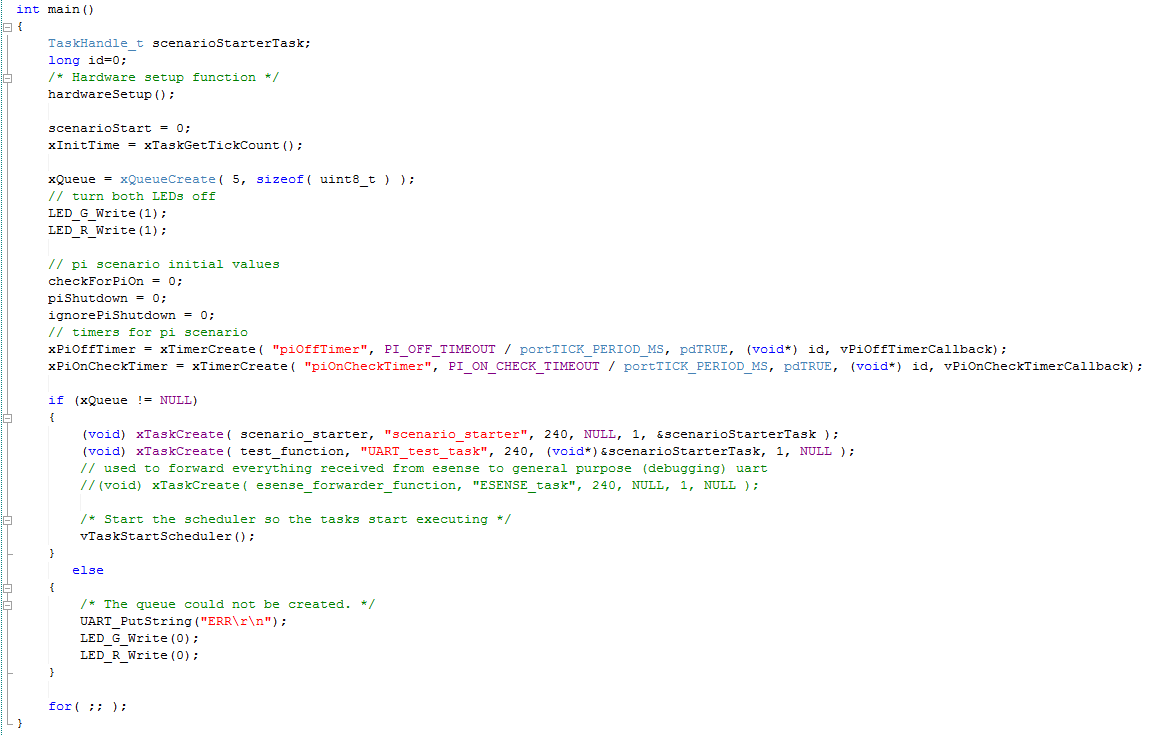
\includegraphics[width=\linewidth]{figures/Main_scenario.png}
	\caption{Main file setup to run a generic scenario}
	\label{fig:main_c}
\end{figure}

\section{Electric sense scenario}

To test electric sense, two different versions of aMussel scenario have been written -- active and passive. 



\end{document}
